\setAuthor{Oleg Košik}
\setRound{lõppvoor}
\setYear{2021}
\setNumber{G 3}
\setDifficulty{3}
\setTopic{TODO}

\prob{Lääts ja ekraan}
Jarl asetas punktvalgusallika ja ekraani vahele õhukese kumerläätse (raamita klaaslääts); valgusallikas asus peateljel ja ekraani tasand oli paralleelne läätse tasandiga. Ta liigutas ekraani edasi-tagasi, uurides sellel tekkivat mustrit ning pani tähele, et kui ekraan asub läätsest kaugusel \SI{10}{\cm}, tekib ekraanile terav valgusallika kujutis. Üllatuslikult selgus, et kui ekraani kaugus läätsest oli \SI{60}{\cm}, siis ei olnud seal näha enam mingit mustrit: ekraan oli ühtlase heledusega nagu läätse polnukski!\\
\osa Leidke läätse fookuskaugus.\\
\osa Mis kujuga muster tekib ekraanile, kui ekraan asub kaugemal, kui \SI{10}{\cm} läätsest, kuid lähemal, kui \SI{60}{\cm} läätsest?



\hint

\solu
\par
\begin{figure}[!h]
  \centering
  \begin{minipage}[c]{0.39\textwidth}
    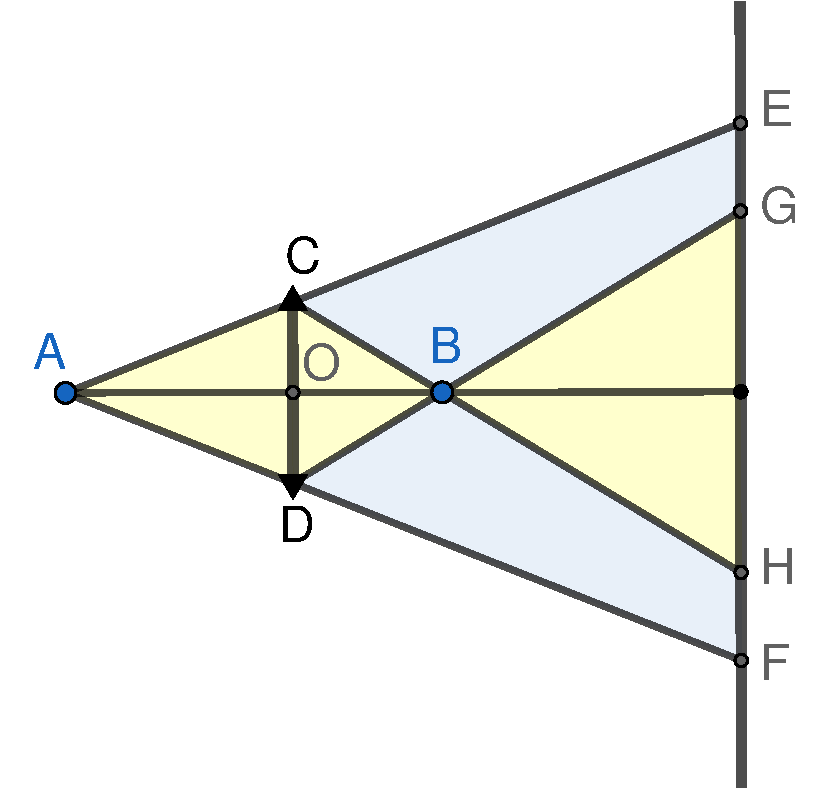
\includegraphics[width=\textwidth]{2021-v3g-03-sol1.pdf}
  \end{minipage}
  \hfill
  \begin{minipage}[c]{0.60\textwidth}
    \vspace*{-2pt}
    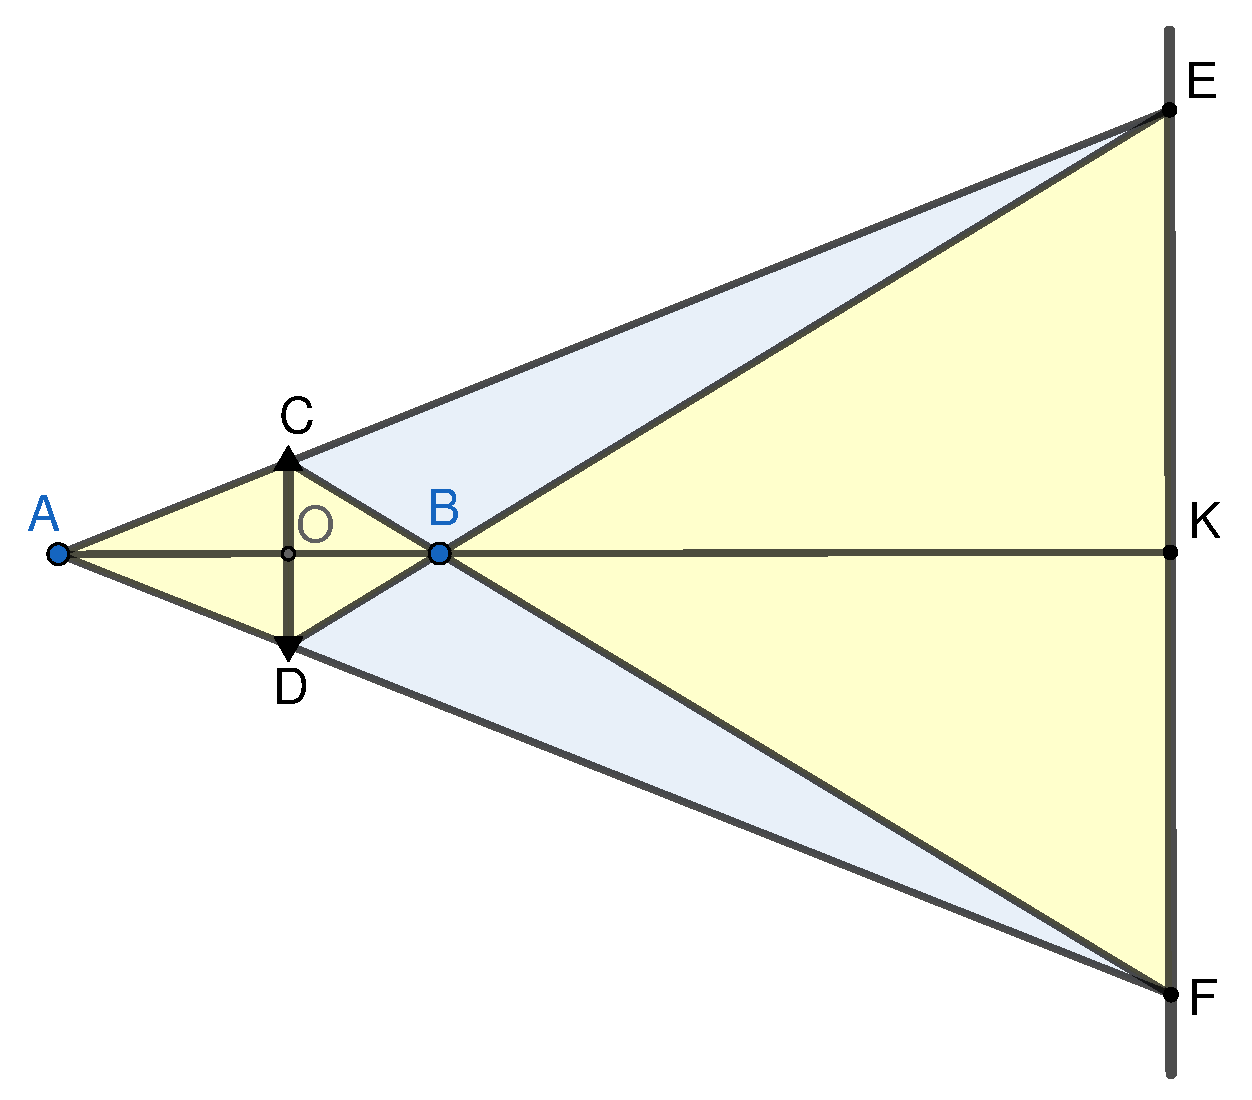
\includegraphics[width=\textwidth]{2021-v3g-03-sol2.pdf}
  \end{minipage}
\end{figure}

Olgu $A$ valgusallikas, $B$ tema kujutis läätses ning $CD$ lääts.

Kui ekraan asub läätsest 10 ja 60 cm vahel, tekivad ekraanile kaks kontsentrilist ringi (vasakpoolne joonis): hele väiksem ring diameetriaga $GH$ asub tumeda ringi diameetriga $EF$ sees. Aladele EG ja HF valgusallika valgus ei jõua.

Eemdaldades läätse ekraanist saavad punktid $E$ ja $G$ kokku üheks nagu ka punktid $F$ ja $H$. Ekraani katab ühtlaselt valgus, nagu läätse poleks (parempoolne joonis).

Olgu $x=|AO|$ kaugus valgusallika ja läätse vahel, $r=|OC|$ läätse raadius ning $R=|KE|$. Ülesande tingimustest $|BO|=\SI{10}{cm}$, $|KO|=\SI{60}{cm}$ ning seega $|BK|=\SI{50}{cm}$. Sarnastest kolmnurkadest $AOC$ ja $AKE$ saame
\[
  \frac{r}{R}=\frac{x}{x+60}.
\]
Sarnastest kolmnurkadest $BOD$ ja $BKE$ aga
\[
  \frac{r}{R}=\frac{10}{50}.
\]
Kokkuvõttes saame võrrandi $\displaystyle{\frac{x}{x+60}=\frac{10}{50}}$, mille lahendiks on $x=\SI{15}{cm}$.

Läätse valemist nüüd
\[
  \frac{1}{10}+\frac{1}{15}=\frac{1}{f}\quad \Rightarrow \quad f=\SI{6}{cm}.
\]
\probend